\section{Systemopbygning}
For at kunne finde krav til dette projekts HiFi-forstærker er det nødvendigt at vælge hvilke blokke denne skal bestå af. I dette projekt er der ikke udelukkende valgt at designe en HiFi-forstærker i sin simpleste form, men også at tilføje funktionalitetsudvidende elementer. Systemets opbygning, med adskilte funktionelle blokke, er illustreret på figur \ref{fig:hififorstaerker_opbygning}. Dette afsnit vil argumentere for og forklare den valgte opbygning. 


\begin{figure}[h]
\centering
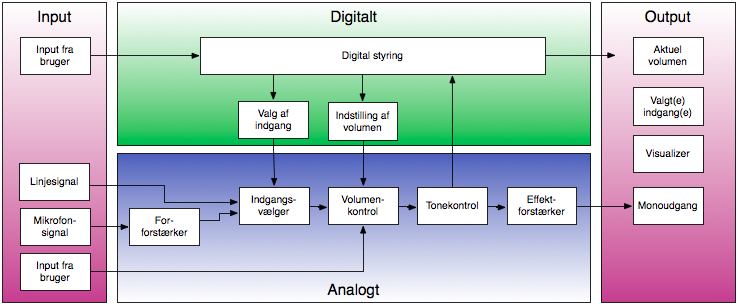
\includegraphics[scale=0.6]{indledende_analyse/systemopbygning/forstaerker_opbygning.png}
\caption{Opbygning af dette projekts HiFi-forstærker}
\label{fig:hififorstaerker_opbygning}
\end{figure}


\subsection*{Input blokke}
Det er valgt at der skal kunne tilsluttes to typer lydkilder til HiFi-forstærkeren; en mikrofon og en kilde som afgiver et liniesignal. Kilder som afgiver et liniesignal er blandt andre computere, de fleste mobiltelefoner og medieafspillere, hvilket er grundlaget for netop at vælge denne type indgang. 
Grundlaget for at vælge en mikrofonindgang er udelukkende for at kunne anvende en indgangsvælger og for ikke at lave to ens linieindgange. Desuden præsenterer en mikrofonindgang en ny blok: forforstærker.

HiFi-forstærkeren skal udstyres med et frontpanel hvorpå alle knapper til justeringsmulighederne skal placeres, således at de er tilgængelige for brugeren. Justeringsmulighederne, som skal være tilgængelige for brugeren er equalizerbånd, volumen og valg af indgang.

\subsection*{Analoge blokke}

Udgangsspændningen fra en mikrofon er langt lavere end linieniveau. Derfor benyttes en forforstærker til at forstærke mikrofonens lave signal op på niveau med liniesignalet, således at de er sammenlignelige i resten af systemet.

For at kunne vælge mellem de to indgange, mikrofon og linie, er det valgt at benytte en indgangsvælger. Indgangsvælgeren skal, foruden at slukke for den ene indgang og tænde for den anden, også kunne tænde for dem begge og dermed blande de to. Det skal, på frontpanelet, være muligt at skifte mellem indgangene samt se hvilke indgange der aktuelt er aktive / inaktive. 

For at kunne skrue op og ned for lydniveauet på HiFi-forstærkeren skal der implementeres en volumenkontrol. Volumen skal kunne justeres på frontpanelet og det skal desuden være muligt at se den aktuelle volumen. \fixme{skal her stå noget om hvor mange niveauer osv?}

Brugeren skal have mulighed for at kunne forme lyden, som HiFi-forstærkeren afgiver. Dette vil blive gjort med en equalizer, hvis funktion er at dæmpe et forudbestemt antal frekvensbånd indenfor hele frekvensområdet. Denne justeringsmulighed af hver enkelt bånd skal være tilgængelig for brugeren på frontpanelet. 

Effektforstærkerens opgave er at levere strøm til højtaleren således at den ønskede afsatte effekt opnås.

\subsection*{Digital styring}
Visse elementer på HiFi-forstærkeren skal styres digitalt. Dette gælder volumenkontrollen og indgangsvælgeren. De digitale blokke vil så vidt muligt, i dette projekt, være designet med gates, da det passer med pensum for det aktuelle semester. 


\subsection*{Output blokke}

For at kunne vise information om aktuelle indstillinger til brugeren vil der bliver benyttet to former for displays. 
Den aktuelle volumen vil blive vist på 7-segment displays. Grunden til valget af 7-segment er for at kunne lave displaydriveren med gates og kunne færdiggøre den over en overskuelig tidsperiode. 

Visning af den aktuelt aktiverede indgang og visualizeren bliver med lysdioder. Da der er to indgange, som kan tændes og slukkes, skal der være to lysdioder, som er tændte hvis indgangen er aktiv. Visualizeren skal have et bestemt antal lysdioder pr. justerbart frekvensbånd, således at jo flere lysdioder der lyser jo højere er lydniveauet på det aktuelle bånd.